% THESIS CHAPTER

\chapter{Software architecture}
\label{chap:sixth
}
\ifpdf
    \graphicspath{{Chapter6/Figures/PNG/}{Chapter6/Figures/PDF/}{Chapter6/Figures/}}
\else
    \graphicspath{{Chapter6/Figures/EPS/}{Chapter6/Figures/}}
\fi

% short summary of the chapter
\section*{Summary}

This Chapter introduces the reader to the software architecture running off board on Linux. The introduction presents a  general overview on software architectures, expressed the needs of such a system and in particular it describes the environment and software tools involved. Next section presents the design pattern according to which the software is organized explaining its advantages and limitations. Then the software components are described with more detail one by one and the results of the experiments are reported. 
\section{Introduction to the proposed architecture}

Architecture is usually intended as the process or product of planning, designing and constructing entities. Usually those entities refer to buildings and structure but the concept can be extended to vehicles, electrical and electronics components or softwares. The architect decides where to locate different elements such as walls, doors columns and windows and connect them in harmony with structural consistency. In the same way the software engineer connect, design and locate different software components. A component could be a program implementing an algorithm, some conversion or a graphical user interface. The basic idea of architecture definition is to design software structure and object interaction before the detailed design phase. Although serious architecture definition is being suggested for large projects only, arguably any software construction or implementation work must be preceded by an architectural design \cite{msdn}.
 \subsection{Motivations}
At this point one may ask: why do we need to define an architecture? The answer is pretty simple: it makes things easier,more clear and simpler. A software architecture is an abstract view of a software system distinct from the details of implementation, algorithms, and data representation. Thus it gives an organizational map we may follow during the design flow. A well written software architecture should:
 \begin{itemize}
 \item Provide flexibility and adaptability.
 \item Allow for interoperability with other softwares and elements in general.
 \item Provide control on the system.
 \item Reduce maintenance time and cost.
 \item Help developers improving the software.
 \end{itemize}
Reusability is a key aspect in design of this kind of systems. One software may be used for a different application changing only few parameters or modules. Each module should be self contained and work as a \textit{black box}, meaning that once the input and output are defined, the actual implementation has no importance. Standardization clearly takes an important role, the way components communicate for example must be known by the developer. If different modules speak the same \textit{language} or \textbf{protocol} (e.g. the MavLink standard) in engineering terms, it is simpler to interface them. Moreover, a self contained module is more easy to maintain and expand because developers can focus on that specific aspect without knowing what is happening outside. In that way specialist in different fields can cooperate designing each own part. The role of the software engineer is on one hand to design software components, and on the other to integrate them with modules written by others. Finally, it seems trivial to point it out, but the architecture must work respecting the specifications and providing the needed control on the system. 

\paragraph{Note:}This software was designed ad-hoc for indoor flight because there were not any other alternatives. Every control station is specialized for outdoor flight which is not our case. Moreover this software aims to become a research platform for controlled environments (e.g. indoor flight) for anyone who wants to contribute.
\subsection{Programming environment and tools}

Every job has its own tools. In order to implement what we theorized in the introduction of this Chapter we need to rely on software tools. There are many different frameworks which helps developers in implementing their own ideas.

 The state of the art and widely used framework in robotics is ROS or Robotic Operative System \cite{ROS}. ROS is a publish/subscrbe middleware meaning that it packs function classes and features which provide inter process communication. It supports most of the libraries used in robotics for path planning, computer vision, control and so on. The main feature is that ROS is very easy to use and let the user create different parallel processes (or nodes) without focusing on low level aspects. As consequence of that, the designer can concentrate on the actual problem he is working on and leave lower level managing such as shared variables, timing or buffers to ROS. This feature increase exponentially the productivity while writing a program. Moreover, ROS is becoming a standard in research and also industry. That means that many packages are available online that one can use, the community and the documentation are superb and it is open source. This framework has all the features needed for a good base of a software architecture.
 
 However there are three main reason which made me discard ROS as a choice. First of all, as stated in Chapter \ref{chap:second}, most of the control stations are written with Qt libraries. Since one may thing to include this architecture in one of them in the future, could be an idea to go in the same direction. The second one is that the very first module of this architecture was written by a PhD student, Tommaso Falchi Delitalia, using the Qt framework. It was nice to have a base starting point and expand from that. The last reason, but not the least, is that ROS gave me important delay problems when I tried to integrate mavlink in it. Mavlink is not fully supported but some packages, in development, are out there and they simplify the design such as the acquisition of data from Motive \cite{optiros}.

Hence the used tools are \textbf{Qt libraries} \cite{qt} while the chosen programming language is C++, widely used and a standard in robotics. Qt is a powerful framework that let the user create user interfaces with good performance. It packs a set of classes, functions and libraries for almost any kind of needs. Moreover is portable on different platforms such as tablets, smartphones and the most important operative systems. for this reason it is used to implement control station, applications like navigators and vehicles control panels.

The functions and classes used for this project are debugging functions to print logs, multi-threading classes to implement parallel modules, sockets interfaces classes and system functions to manage lower level services.By far Qt seems perfect, it provides a very easy access to many features, the documentation is very clear and the learning time is pretty low. The very big disadvantage is the lacking of inter process communication support. The pub/sub design is perfect for robotics application but Qt does not provide any help on that, at least for now. Thus the drawbacks of using this kind of framework is that we need to manage inter process message pass-through in some way. This is done and explained in section \ref{sec:sofdescrip}. A porting on ROS could be interesting in the future, after solving delay related issues, for research interests.
\section{Design patterns}
\label{sec:patterns}
In the course of history the concept of \textit{style} was born and developed. An architectural style is characterized by the features that make a building or other structure notable and historically identifiable. The style identifies a common trend, elements or rules that are used in a particular period or by a group of people during the design flow. The same concept evolved to various disciplines; in computer science, the architecture "style" is often called \textbf{Design Pattern}. The analogy with building design is strong, the formal definition of design pattern is the following: 
\paragraph{Definition of Design Pattern}:  \textit{a design pattern is a general reusable solution to a commonly occurring problem within a given context in software design.} \\

\noindent
The pattern is a description or template for how to solve a problem that can be used in many different situations, usually for groups of problems. Similarly to the architecural style, the software pattern is defined by common structures, participants, communications, protocols and standards. Design patterns can speed up the development process by providing tested, proven paradigms. Thus the software architecture is defined by its style, namely design pattern, which is chosen among the available ones. First step to follow during the prototyping of the software is to have clear in mind which kind of problem we are facing and which are the constraints of the system. 

At this point the reader should ask how is the software interfacing with the robot and which kind of control does it have on the system. As stated in Chapter \ref{chap:fifth}, the external signals that are input of the on board flight stack are the 4-D position value from the mocap and the 4-D position set point. By 4-D we mean a vector composed with [x, y, z, yaw] since roll and pith are estimated on board (see figure \ref{figure:controlarch}). Moreover the following goal is set:
\paragraph{Goal:} \textit{The robot must be able to perform some kind of tasks provided by the user in the most autonomous way possible.} \\

\noindent
In other words, the user provides a list of tasks he wants to perform with the robot and the software architecture guide the system by sending mocap values and position set points. The first scheme of the software is represented in figure \ref{figure:inout}. 
\begin{figure}[h]
\centering
 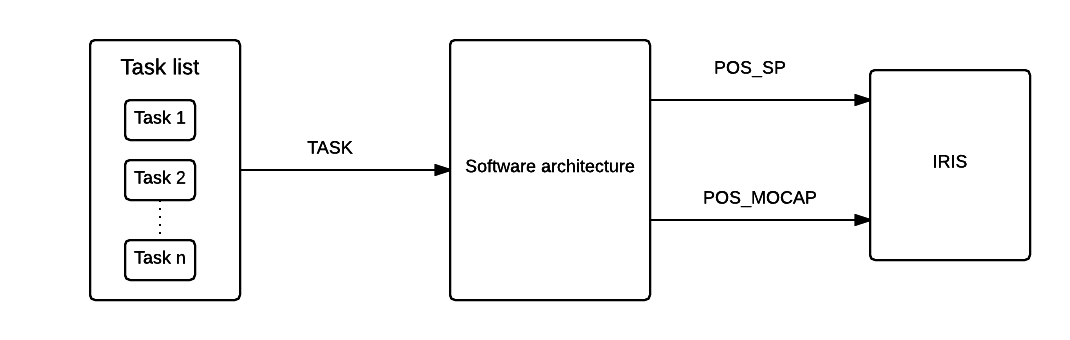
\includegraphics[width=0.8\textwidth]{first_arch.png}
 \caption[In-out relation]{Input / Output relation of the software architecture.}
 \label{figure:inout}
\end{figure}
The scheme explains the input output relation, where as input there is a C-struct describing the task and as output MavLink messages for mocap estimate and position set point. Nevertheless, the real structure is a bit different. I decided to put the task list inside the software architecture as a nested component. The main reason for that is simplicity, in the future one may encode the list in a text file as input of the software. See figure \ref{figure:inoutnest} for the actual implementation.

\begin{figure}[h]
\centering
 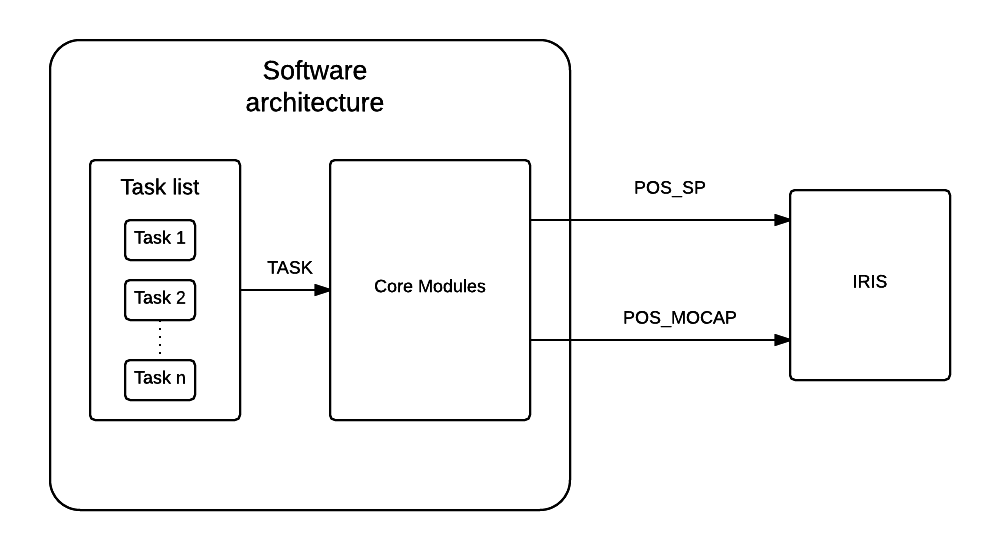
\includegraphics[width=0.8\textwidth]{nested_arch.png}
 \caption[In-out relation for the nested arch]{Input / Output relation of the software architecture with nested component.}
 \label{figure:inoutnest}
\end{figure}

\subsection{Behavioral architecture}
At this point, a way to model the problem is necessary. Let us start from the goal: there a list of tasks and the robot must executes them sequentially and autonomously. Thus, the concept of task arises. The task is defined as \textit{a definite piece of work assigned to the robot and performed by acting on the environment}. 

\paragraph{Defined tasks} Which kind of tasks may be performed by IRIS? The first step is to define the essential tasks of navigation which are:
\begin{itemize}
\item Take off - from the ground or an horizontal plane.
\item Land - land on actual position.
\item Move - go to a target point in 3-D space.
\item Rotate - Change yaw value to a desired one.
\item Follow trajectory - Perform a circle around an arbitrary center set in the parameters.
\end{itemize}
Moreover a fifth task is added but discussed in \ref{chap:seventh} which is land on a mobile platform. \newline \\
In order to make things more flexible, each task has a set of parameters used to influence the performance during the execution and to adapt to the environment. A detailed explanation is given in \ref{sec:auto}. Furthermore, it is evident that most of the tasks described involve in some way a location in space. Hence the task is modeled in a C-struct with two elements: position and action. In the software the task takes the name \textbf{node} which is often used in control stations and graph based applications.

Table \ref{tab:node} describes the node struct. The position \textit{p} is itself a struct with four elements (x,y,z,yaw) encoding the 4-D pose in space. The action \textit{a} is another stuct with a char value to identify the type of action and a parameter array which can be filled with values. The meaning of the parameter array changes depending on the action.
\begin{table}[h]
\centering
\begin{tabular}{llll}
\multicolumn{4}{c}{\textbf{Node} struct} \\
\hline
position \textit{p} &     &       &           \\
           & \textit{x}   & double & meters    \\
           & \textit{y}   & double & meters    \\
           & \textit{z}   & double & meters    \\
           & \textit{yaw} & double & radiants  \\ \hline
action \textit{a}   &     &       &           \\
           & \textit{id}  & char  &           \\
           & \textit{params}    &  double[4]     & \\
\end{tabular}
\label{tab:node}
\caption{Node struct descripton}
\end{table}
Those elements are necessary in order to choose which design pattern is suitable in this environment.
\newline \\
\noindent
Taking inspiration from biology and observing how simple animals interacts with the environment, robotic schemes and models may be derived. Biologist discovered that animals like frogs, pigeons insects and fishes exhibit different behaviors depending on the sensory inputs they receive from the environment. With this simple method they are able to survive, hunt and navigate. Two different examples explain the concept very well.

Frogs eyes are able to detect movement. In particular on layer detects small moving objects like flies and another layers detects big object, for example predators. The two layers work in parallel. When the first one is activated, meaning that there is food in the proximity, the frogs jumps towards the pray. On the other hand, when the second layer is triggered, the frogs run away from the object. 

The second example involves the navigation of pigeons. When it is sunny, the bird uses the sun to locate himself (behavior 1). When it is cloudy they use the magnetic field of the earth to detect the north (behavior 2). By disturbing the pigeon with artificial light, it get confused only in sunny days. Vice versa, if disturbed with a magnet, it get confused only in cloudy days. This simple experiment lead to an important result: the pigeon switch behavior depending on some triggering inputs just like the frog. More over only one behavior is active. 
\paragraph{Behavior definition} \textit{A behavior is a mapping of sensory inputs to a pattern of motor actions that are used to achieve a task.} \newline

\noindent
For the frog, the sensory inputs are be the position of the moving objects while for the pigeon they are the position of the sun and the value of the magnetic field. Moreover, a trigger is present. Those triggers are of different nature depending on the animal, they activate the behaviors or switch from one to the other. Figure \ref{figure:behavior} shows the basic model of the behavior. Inputs and output may be more than one while the activation trigger is always a single signal. 
\begin{figure}[h]
\centering
 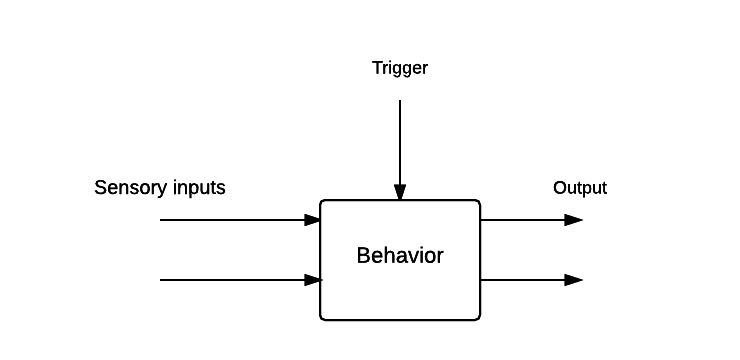
\includegraphics[width=0.8\textwidth]{behavior.png}
 \caption[Behavior definition]{Scheme of the behavior.}
 \label{figure:behavior}
\end{figure}
From an engineering point of view, imagine the behavior like a process, an algorithm, a thread or a module. Inputs and outputs may be variables, signals or parameters. The triggers are often booleans. The logic that manage the triggers is called \textbf{switching logic} and it is a key aspect in the architecture. The switching logic is usually a module that takes inputs from perception modules, and outputs the boolean values of each trigger. Figure \ref{figure:switch} describes a behavioral machine, n behaviors are connected to n trigger signals coming out from the switching module. The logic can be implemented in different ways. It could be a combinatorial circuit made by logical ports, some mathematical functions or a state machine but its output must be a set of n boolean values. 
\begin{figure}[h]
\centering
 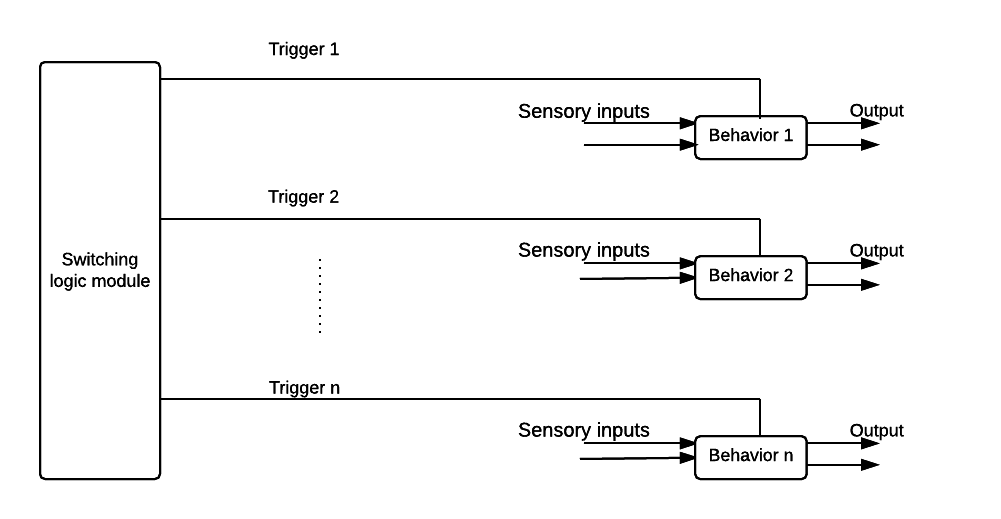
\includegraphics[width=0.8\textwidth]{switch.png}
 \caption[Switching logic]{Behavioral system with switching logic.}
 \label{figure:switch}
\end{figure}

\paragraph{Concurrent behaviors} One aspect I find very interesting is the concept of concurrent behaviors. Two or more behaviors are concurrent when they are active at the same time. This approach may solve elegantly different problems but we must pay some attention. Imagine the frog looking around. At some point an insect and a predator appear together in the field of view activating two behaviors. She is hungry, but more important, she does not want to be the meal of someone else. In this case behaviors can be prioritized (the most important is executed). A second way is to include this scene in the switching logic where behaviors inhibit others. Moving may inhibit landing for example. 

On the other hand let us picture the following situation: a mobile robot moving on the ground and going towards a target. The behavior \textit{move straight} is activated and the robot goes in the direction of the goal. At certain point the perception module senses an obstacle in front and activates the behavior \textit{avoid obstacle}. The two behaviors are concurrent since we assume that there is no inhibition in the switching logic. The first output is to spin the wheels with the same speed (move straight) but the second behavior commands the steering wheels to turn and avoid the collision. The to outputs add up and the result is the robot avoiding the obstacle. When the perception module does not sense anymore the obstruction, the second behavior is turned off and the robot continues moving towards the target. 

It seems pretty trivial but this approach has a lot of potential. It saves resources turning off and on different modules depending on the situation. Switching logic can be implemented on hardware thus optimizing the performances. Moreover the combinations of simple behaviors may solve complex tasks. 

For this case, in order to solve concurrency issues, I used a simple rule: \textbf{concurrent behaviors are possible only if they act on different dynamics}. For example, move and rotate can be activated together because one changes x, y and z while the other changes yaw set points. Follow trajectory and move cannot be concurrent because they act on the same dynamics. One may need to follow a trajectory, like a circle around a point of interest, and film with the camera the center thus keeping the nose always pointing to the target. This is solved combining \textit{follow trajectory} with \textit{rotate}. Although it is not implemented in this way, potentially the landing on a mobile platform task may be defined by two concurrent behaviors. The first is \textit{move} or track the platform, and the second is \textit{land}. The more behaviors are added, the more combinations are possible.

\paragraph{Implementing behaviors} The switching logic is implemented as a finite state machine which is presented in section \ref{sec:exec}. Behaviors are functions with the following inputs: the robot state (x,y,z,yaw), the actual position setpoint(x,y,z,yaw) and the node value. As output they give the new position setpoint which is updated. Figure \ref{chap:fifth} shows the data flow for general set of behaviors, the switching logic is not shown for simplicity. 
\begin{figure}[h]
\centering
 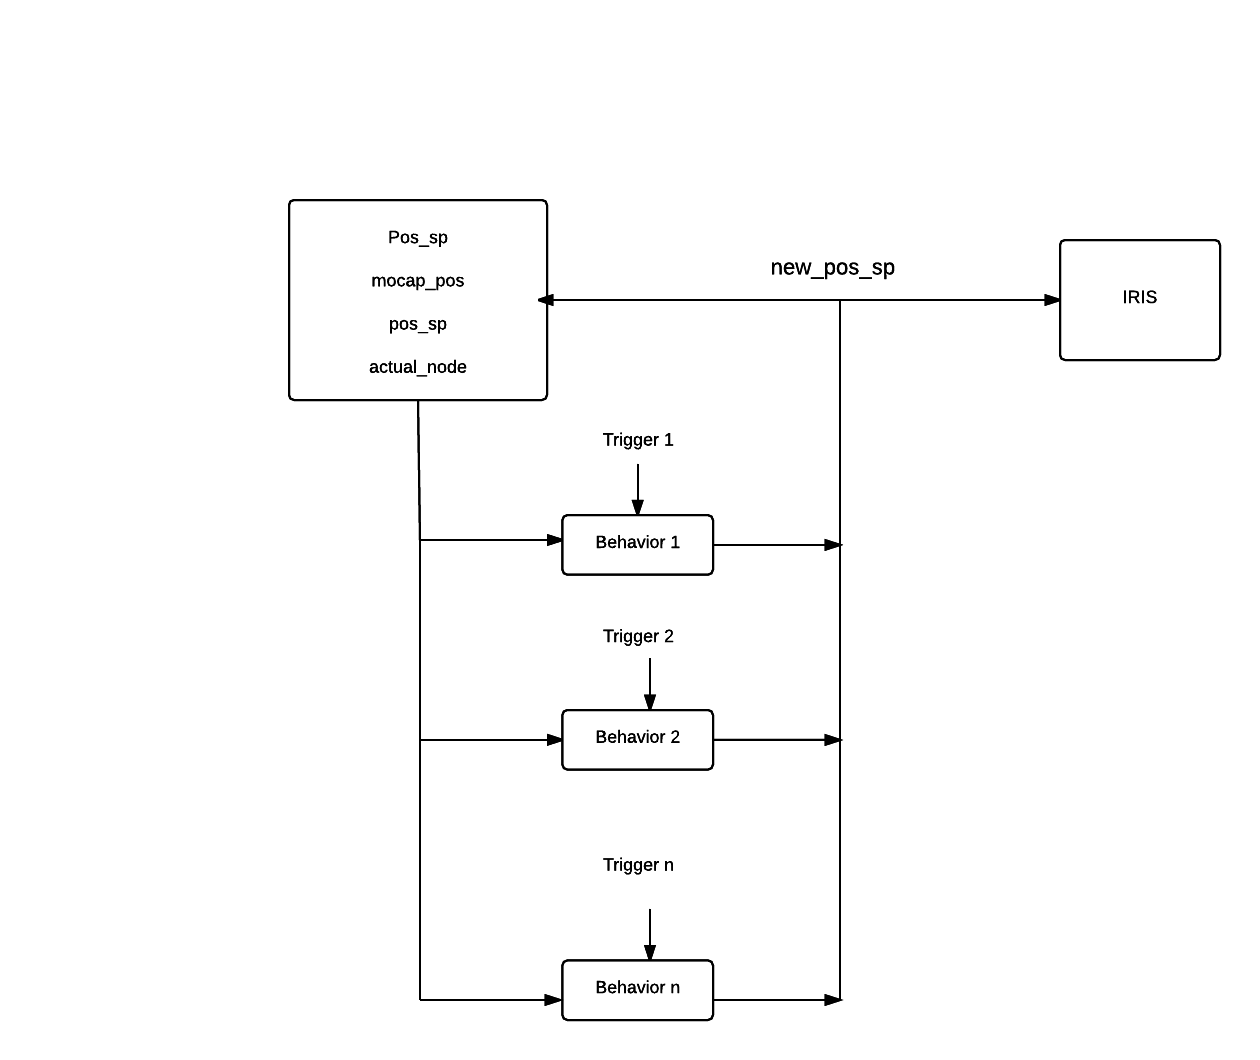
\includegraphics[width=0.8\textwidth]{behav_flow.png}
 \caption[Behavior data flow]{Input/Output relations with particular adopted scheme. Switching logic is not depicted.}
 \label{figure:flow}
\end{figure}
Regarding implemented behaviors, the switching logic is almost a one to one map. Each presented task has its own behavior called with the same name. In this version of the software, the only concurrency appears in \textit{follow trajectory} task which performs a circle and keeps the nose always at the center. Depending on the actual task, the switching module activates different behaviors and the map is shown in table \ref{tab:map}.
\begin{table}[h]
\centering
\begin{tabular}{l|c}
Actual task               & Activated behaviors   \\ \hline
take off                  & take\_off             \\
land                      & land                  \\
move                      & move                  \\
follow trajectory         & follow\_traj ; rotate \\
rotate                    & rotate                \\
land on a mobile platform & plat\_land           
\end{tabular}
\caption{Switching logic mapping.}
\label{tab:map}
\end{table}

For prototyping and simplicity reasons, the mobile landing has its own behavior but two concurrent behaviors can be assigned to it, namely \textit{move} and \textit{land}. Moreover, many improvements can be done. For example one can decide to activate or not the \textit{rotate} behavior in the follow trajectory task by passing a value in the params array. This architecture can be largely expanded from its actual state by adding behaviors, concurrencies and tasks.



\section{Software description}
\label{sec:sofdescrip}

\subsection{General scheme}
\subsection{Service modules}
\subsubsection{NatNet Reciever}
\subsubsection{Position Dispatcher}
\subsection{Manual Control}
\subsection{Automatic Control}
\label{sec:auto}
\subsection {Executioner}
\label{sec:exec}

\section{Experiments and results}